\IEEEPARstart{O}{ver} the past few decades, artificial intelligence (AI) has undergone remarkable advancements, emerging as a transformative technology in diverse domains, including image classification and autonomous systems~\cite{mnih2015human, 8103164}. Among various AI paradigms, deep reinforcement learning (DRL)—which integrates deep learning with reinforcement learning—has emerged as a powerful model-free approach for sequential decision-making in complex, uncertain environments.

\begin{figure}[htbp]
  \centering
  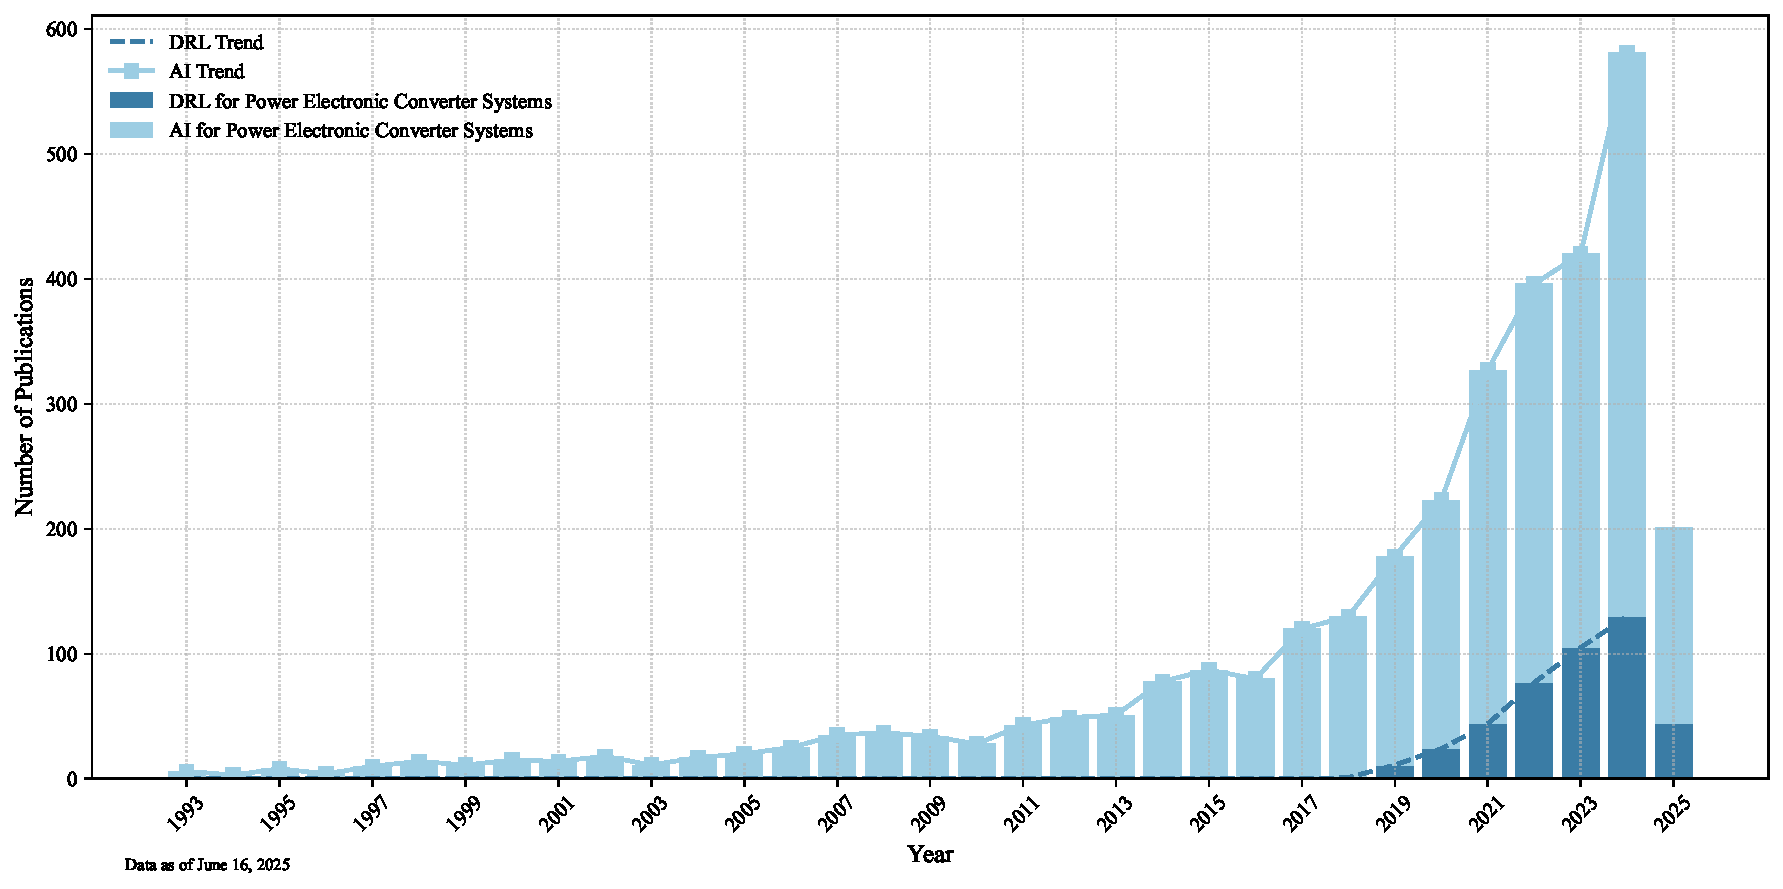
\includegraphics[width=\linewidth]{fig/AI_Stacked_Above_DRL.pdf} 
  \caption{Annual number of publications on AI and DRL in power electronic converter systems since 1993.}
  \label{fig:AI_Stacked_Above_DRL}
\end{figure}

DRL's ability to learn control policies through continuous interaction with dynamic environments shows growing promise in PECs, especially in scenarios requiring adaptive, data-driven intelligence. For instance, the control of LCL-filtered grid-tied inverters suffers from resonance instability and parameter sensitivity, where traditional proportional-integral (PI) or model predictive controllers often require extensive tuning and precise system modeling. In contrast, DRL can autonomously learn optimal switching or modulation policies through environment interactions, mitigating the need for accurate models. Similarly, in renewable energy systems such as photovoltaics (PV) and wind power, maximum power point tracking (MPPT) must contend with rapidly changing environmental conditions; DRL-based MPPT controllers have demonstrated superior adaptability and tracking accuracy under such non-stationary inputs~\cite{8991860, 9721402}. These examples highlight how DRL's model-free, policy-optimization capabilities naturally align with the nonlinear, time-varying dynamics of PECs.

Building on these capabilities, DRL has been increasingly applied to a broad range of converter-related tasks, including MPPT, modulation control, power quality enhancement~\cite{8991860, 10424981, 10197504}, topology optimization~\cite{9841555, 9950526}, and predictive maintenance (PM) functions such as condition monitoring, anomaly detection, fault diagnosis, and remaining useful life (RUL) estimation~\cite{10423410, 9528837, 10616165}. These developments position DRL as a key enabling technology for intelligent and autonomous PECs across their full lifecycle.

Advancements in sensor networks, the Internet of Things (IoT), edge computing, and digital twin technologies~\cite{8281479, 9139976, 11005593} have enhanced system observability and data availability. These technologies enable the collection of heterogeneous operational data—such as voltage, current, switching states, and environmental conditions—which can be used for real-time design optimization, adaptive control, and maintenance decision-making~\cite{8906073}. As shown in Fig.~\ref{fig:AI_Stacked_Above_DRL}, research interest in AI, particularly DRL, for PECs has surged in recent years.

\begin{figure}[htbp]
  \centering
  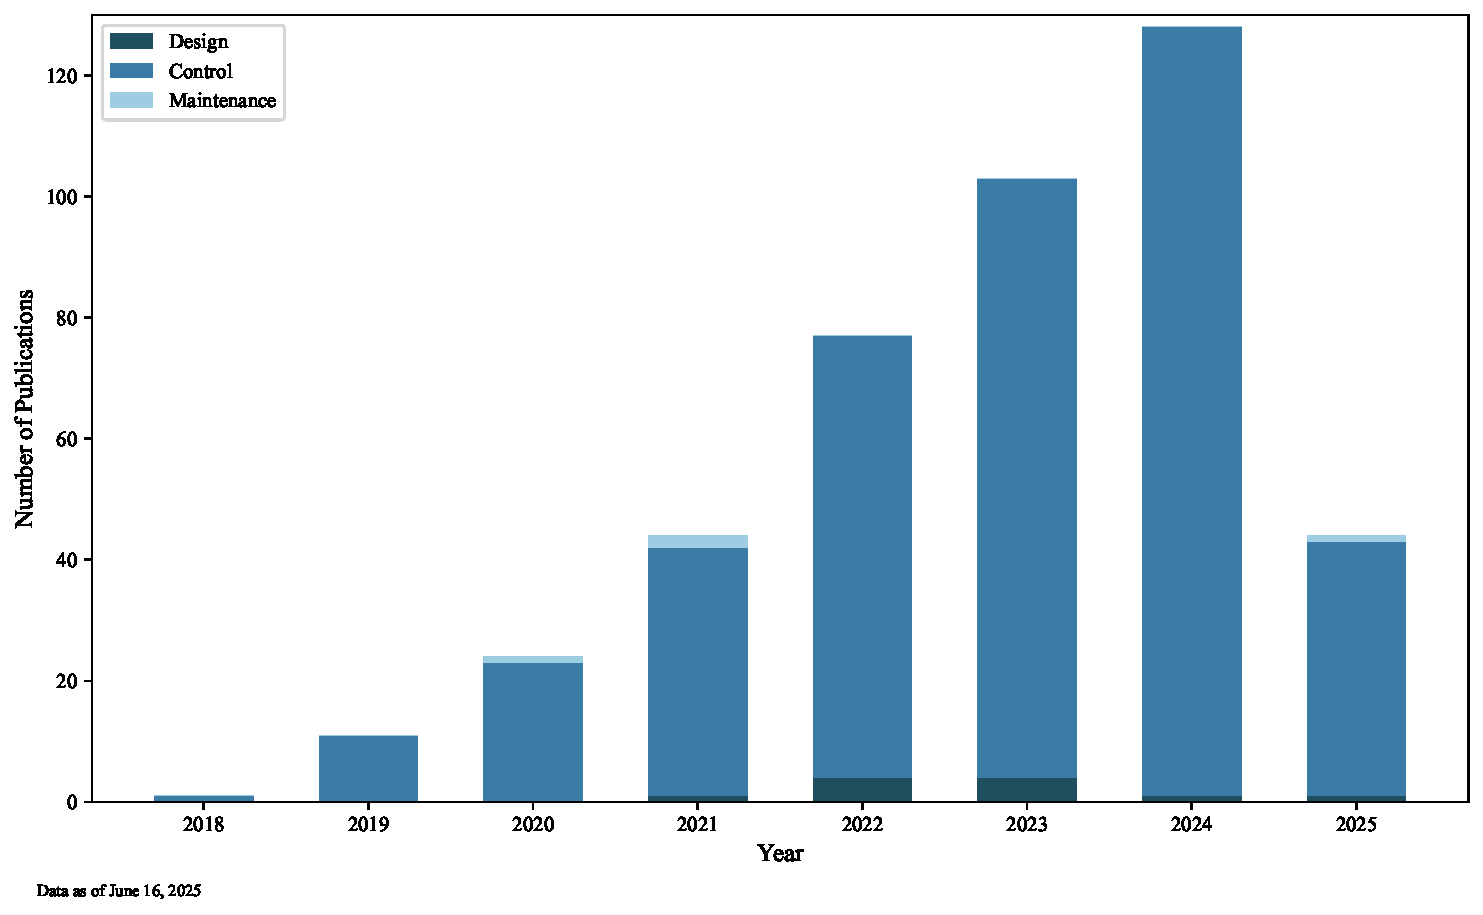
\includegraphics[width=\linewidth]{fig/DRL_Task_Distribution.pdf}
  \caption{Distribution of DRL-related publications across design, control, and maintenance tasks in PECs.\\
  \textit{Data Source: Google Scholar, filtered by the keywords "deep reinforcement learning", "power electronic converter systems", and domain-specific task terms. Full publication list is provided in the supplementary material.}}
  \label{fig:DRL_Distribution}
\end{figure}

Fig.~\ref{fig:DRL_Distribution} shows the distribution of 436 DRL-related publications (from 2018 to 2025), categorized by task domain. These publications were curated from the Web of Science Core Collection, focusing on peer-reviewed journals and flagship conferences in power electronics and intelligent systems. Prominent venues, such as IEEE Transactions On Power Electronics (TPEL), IEEE Transactions On Industrial Electronics (TIE), and IEEE Energy Conversion Congress and Exposition (ECCE), are widely recognized for publishing high-impact research in converter technologies and AI-enabled control systems. The full publication list is available in the supplementary material. As shown in Fig.~\ref{fig:DRL_Distribution}, control-related applications dominate, accounting for over 95\% of all DRL studies in PECs. However, publications on design optimization and PM have shown a certain growth trend since 2021, reflecting an expanding research focus from low-level control to system-wide lifecycle intelligence. This trend reflects a growing recognition of DRL's potential across the entire PECs lifecycle, from early-stage design to long-term operation and maintenance.

Despite this momentum, most existing reviews either provide broad surveys of AI in power systems~\cite{10336908, 9200511} or focus on specific DRL use cases (e.g., renewable energy~\cite{9721402}, smart grids~\cite{8859593}, or converter control~\cite{10613457}). These reviews lack a unified DRL-centered framework spanning multiple stages of the PEC lifecycle and fail to address algorithmic trade-offs, implementation bottlenecks, and future research opportunities.

To bridge this gap, this article presents a comprehensive and structured review of DRL applications across the full lifecycle of PECs. Emphasizing the domains of design optimization, intelligent control, and PM, the key contributions of this work are:

\begin{itemize}
  \item[1)] A taxonomy of DRL algorithms applied to converter systems, covering value-based, policy-based, actor-critic, and multi-agent methods such as deep Q-network (DQN), deep deterministic policy gradient (DDPG), twin delayed deep deterministic policy gradient (TD3), proximal policy optimization (PPO), soft actor-critic (SAC), and multi-agent deep deterministic policy gradient (MADDPG).
  \item[2)] A lifecycle-oriented classification of DRL applications in PECs, structured around three core domains: design optimization, intelligent control, and PM.
  \item[3)] A critical discussion of practical implementation challenges for DRL in converter hardware, including sample efficiency, safety constraints, policy interpretability, and embedded deployment scalability.
  \item[4)] A forward-looking analysis of emerging opportunities, such as physics-informed reinforcement learning (RL), explainable DRL, multi-agent coordination, and real-time adaptation for robust and autonomous PEC operation.
\end{itemize}

The rest of the article is organized as follows. Section~II introduces DRL fundamentals, algorithm classes, and milestones in PECs applications. Sections~III to~V review DRL applications in design optimization, intelligent control, and PM, respectively. Section~VI discusses limitations and future opportunities. Section~VII concludes the paper.



